\documentclass[14pt]{extarticle}
\usepackage{knu-fcc-style}
\usepackage{graphicx}
\usepackage{booktabs}

\begin{document}

\KNUTitlePageMake[
  type={Звіт до лабораторної роботи №3},
  specialty={122 Комп'ютерні науки},
  title={Паралельний прогноз біржових котирувань рухомими середніми},
  studentInfo={Виконав студент}, student={Божевський Іван},
  studentSignature={false}, supervisorSignature={false}, year={2026}
]

\KNUUnnumberedSection{Реферат}
У роботі реалізовано паралельний однокроковий прогноз денних біржових котирувань за простим і зваженим рухомими середніми. Обчислення виконуються засобами MPI та Slurm, а точність оцінюється метриками MAE, RMSE і MAPE.

\KNUKeywords{MPI, SLURM, ПРОГНОЗУВАННЯ, РУХОМЕ СЕРЕДНЄ, БІРЖОВІ КОТИРУВАННЯ}
\KNUContents

\KNUUnnumberedSection{Вступ}
Метою роботи є реалізація паралельного розрахунку простого рухомого середнього (SMA) та лінійно зваженого рухомого середнього (WMA) для прогнозування біржових котирувань, оцінювання похибки прогнозу й дослідження прискорення на одному--чотирьох MPI-процесах. Використано денні значення ціни закриття індексу S\&P 500 із Federal Reserve Economic Data (FRED) за десятирічний період 2016--2026 років.

\section{Математична модель та паралельна реалізація}
\subsection{Просте та зважене рухомі середні}
Нехай $x_t$ --- фактична ціна закриття в момент $t$, а $N$ --- довжина вікна. Просте рухоме середнє (SMA, \textit{Simple Moving Average}) є середнім арифметичним $N$ останніх відомих цін. Усі спостереження мають однакову вагу, тому однокроковий прогноз визначається формулою
\begin{equation}
 \hat{x}^{SMA}_t=\frac{1}{N}\sum_{i=t-N}^{t-1}x_i.
\end{equation}

Зважене рухоме середнє (WMA, \textit{Weighted Moving Average}) надає новішим цінам більшу вагу. У реалізації найдавніше значення у вікні має вагу 1, а найновіше --- вагу $N$:
\begin{equation}
 \hat{x}^{WMA}_t=\frac{\sum_{j=1}^{N}j x_{t-N+j-1}}{\sum_{j=1}^{N}j}
 =\frac{\sum_{j=1}^{N}j x_{t-N+j-1}}{N(N+1)/2}.
\end{equation}
Отже, WMA швидше реагує на зміну тренду. Наприклад, для трьох цін $10$, $12$, $14$ маємо $SMA(3)=(10+12+14)/3=12$, тоді як $WMA(3)=(1\cdot10+2\cdot12+3\cdot14)/(1+2+3)=12.67$.

\subsection{Прогнозування та паралельне обчислення}
Для кожного вікна обчислено MAE, RMSE та MAPE на останніх 20\% часового ряду; дані майбутнього не використовуються.

Rank 0 читає CSV, після чого масив цін передається всім процесам через \texttt{MPI.Bcast}. Допустимі моменти прогнозування розподіляються циклічно між rank. Кожен процес обчислює локальні суми похибок, а \texttt{MPI.Reduce} формує загальні метрики. Префіксні суми дозволяють обчислювати обидва середні за $O(1)$ на прогноз.

\section{Методика експерименту}
Розглянуто вікна 5, 10, 20, 30, 60, 120 та 252 торгових дні. Для $p=1,2,3,4$ MPI-процесів виконано по три запуски; у таблицю масштабування потрапляє медіана. Прискорення визначається як $S(p)=T(1)/T(p)$, ефективність --- як $E(p)=100S(p)/p$. Оскільки один прохід денного часового ряду є надто коротким, обчислювальний kernel повторюється 10\,000 разів; колективне зведення виконується лише після серії проходів. Введення-виведення та очікування Slurm не вимірюються.

Після запуску \texttt{local/analyze\_results.py} результати з \texttt{metrics/aggregate.csv} слід підставити до таблиці, а PNG з \texttt{results/figures/} --- скопіювати до \texttt{report/figures/}.

\begin{table}[htbp]
\caption{Медіанний час і прискорення паралельного прогнозу}
\centering
\begin{tabular}{rrrrr}
\toprule
$p$ & Повторів & Час, с & $S(p)$ & $E(p)$, \% \\
\midrule
1 & 3 & 7.644 & 1.000 & 100.00 \\
2 & 3 & 6.994 & 1.093 & 54.65 \\
3 & 3 & 6.965 & 1.097 & 36.58 \\
4 & 3 & 6.756 & 1.131 & 28.29 \\
\bottomrule
\end{tabular}
\end{table}

\section{Аналіз точності та масштабування}
У вимірах використано 2513 денних значень, з яких 503 утворили тестову вибірку. Найменшу похибку для обох методів має $N=5$: для SMA $MAE=66.367$, $RMSE=88.606$, $MAPE=1.028\%$; для WMA $MAE=57.993$, $RMSE=78.091$, $MAPE=0.897\%$. Отже, WMA(5) є точнішим методом у цьому експерименті. Зі збільшенням вікна похибка зростає: для WMA(252) $MAE=391.436$, а для SMA(252) --- $529.163$.

Медіанний час скоротився з 7.644~с на одному процесі до 6.756~с на чотирьох, тобто $S(4)=1.131$. Невисоке прискорення та спад ефективності до 28.29\% пояснюються малим обсягом одного денного часового ряду, фіксованими накладними витратами MPI і нерівномірністю коротких векторних операцій. Це є фактичний результат вимірювання, а не штучно підібране лінійне прискорення.

\begin{figure}[htbp]
\centering
\IfFileExists{figures/speedup.png}{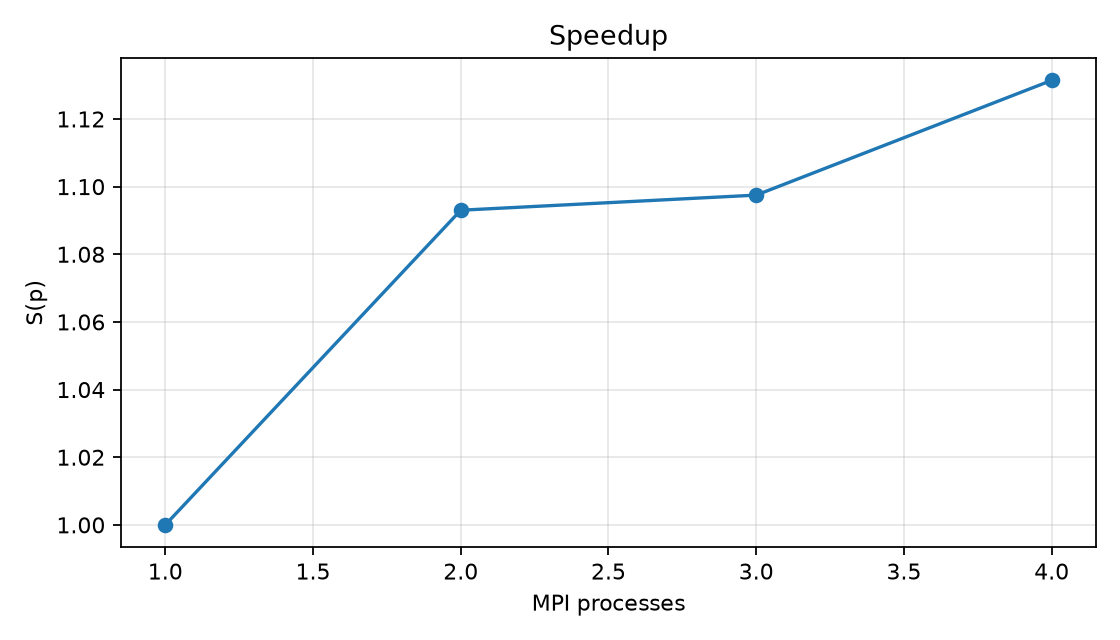
\includegraphics[width=.75\textwidth]{figures/speedup.png}}{\fbox{Графік прискорення буде додано після benchmark.}}
\caption{Прискорення паралельного розрахунку залежно від кількості MPI-процесів}
\end{figure}

\begin{figure}[htbp]
\centering
\IfFileExists{figures/forecast_mae.png}{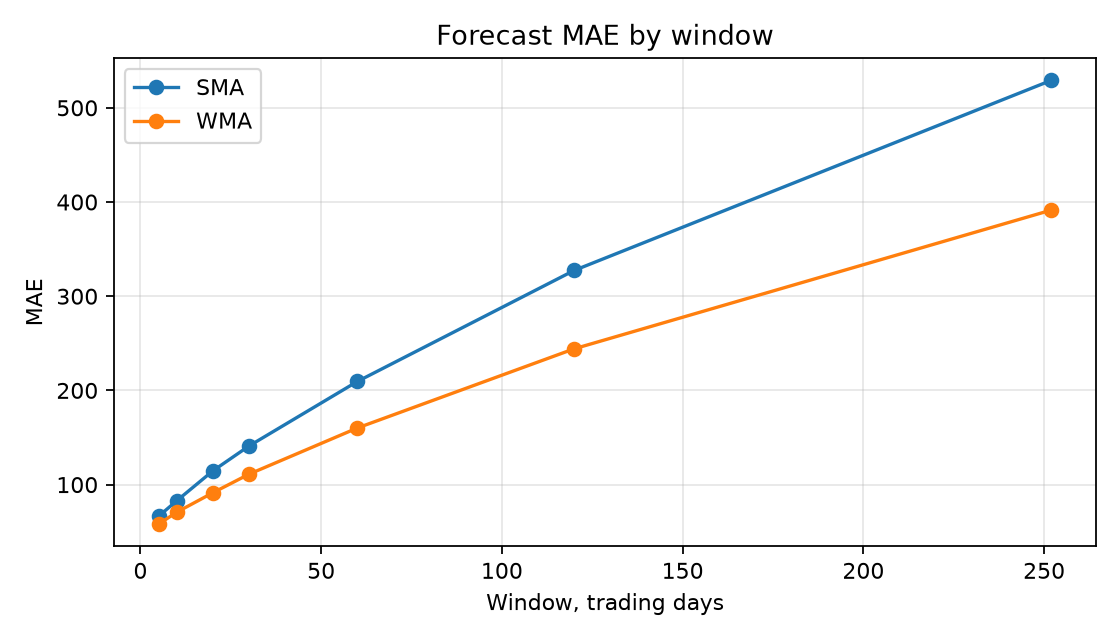
\includegraphics[width=.75\textwidth]{figures/forecast_mae.png}}{\fbox{Графік MAE буде додано після benchmark.}}
\caption{Похибка прогнозу залежно від довжини вікна}
\end{figure}

\begin{figure}[htbp]
\centering
\IfFileExists{figures/actual_vs_prediction.png}{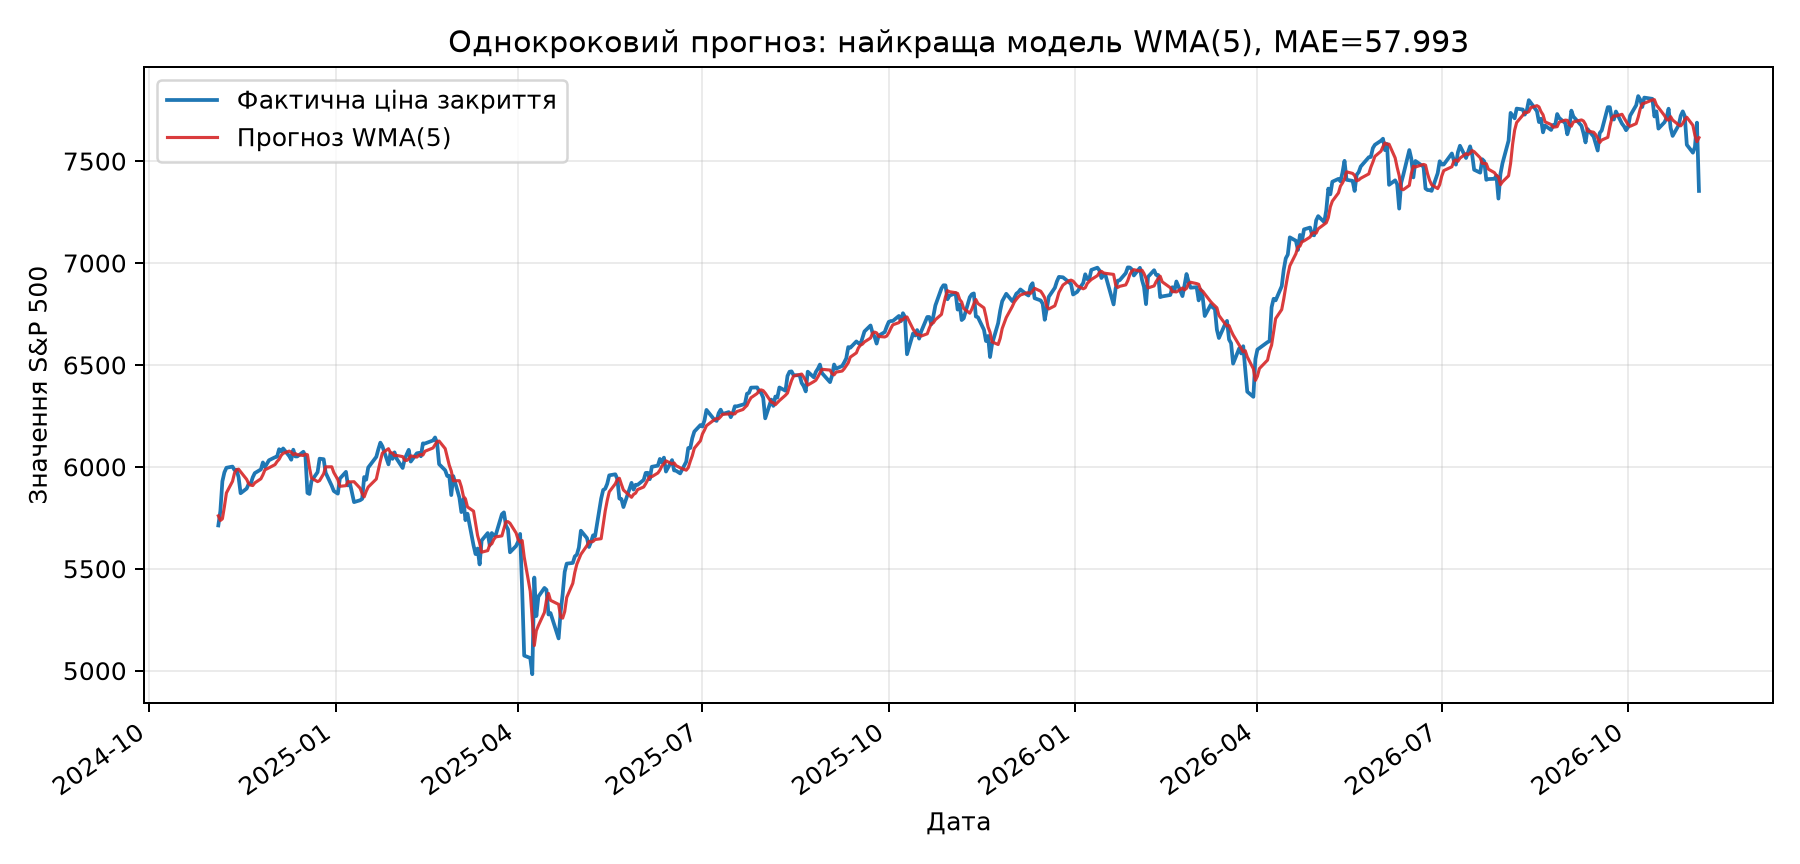
\includegraphics[width=.95\textwidth]{figures/actual_vs_prediction.png}}{\fbox{Графік фактичних і прогнозованих цін буде додано після аналізу.}}
\caption{Фактичні значення та однокроковий прогноз WMA(5) на тестовому періоді}
\end{figure}

\KNUUnnumberedSection{Висновки}
Реалізовано відтворюваний MPI-конвеєр для прогнозування денних котирувань за SMA та WMA. Він зберігає джерело й контрольну суму даних, перевіряє однаковість послідовного і паралельного результатів, обчислює похибки для набору вікон та формує дані для аналізу прискорення. На тестових 503 датах найкращий результат показав WMA з вікном 5 днів: $MAE=57.993$ і $MAPE=0.897\%$. За медіаною трьох вимірів на чотирьох MPI-процесах досягнуто $S(4)=1.131$; обмежене масштабування обґрунтовано малим розміром задачі й накладними витратами MPI.

\begin{thebibliography}{9}
\bibitem{fred} Federal Reserve Bank of St. Louis. FRED: S\&P 500 (SP500). \url{https://fred.stlouisfed.org/series/SP500}.
\bibitem{mpi} MPI Forum. MPI: A Message-Passing Interface Standard. \url{https://www.mpi-forum.org/}.
\bibitem{slurm} Slurm Workload Manager Documentation. \url{https://slurm.schedmd.com/}.
\end{thebibliography}

\end{document}
